\chapter{The renormalization group}
After the renormalization of QED, the systematics of the procedure and consequences on physical observables were still not fully understood. Between the Fifties and the Seventies there were several studies of how residual scale dependence on renormalized quantities in perturbation theory implied evolution equations for the model parameters. The first works were by Stuckelberg, Petermann, Gell-Mann and Low studying electric charge in QED. The ideas were formalized in the works of Callan, Symanzik, and Wilson. 

\section{Scale dependence of electric charge}
We can use the result for $\Pi^{\mu\nu}$ at 1-loop to study the electric charge at different scales. Recall that the vacuum polarisation in QED was
\begin{equation}
    \tilde{G}^{\mu\nu}(q^2,\dots) = -\frac{ig^{\mu\nu}}{q^2}\frac{1}{1 + \Pi(q^2,\alpha,m^2)} + \tilde{G}_L^{\mu\nu}(q^2,\dots).
\end{equation}
$\Pi(q^2,\alpha,m^2)$ was renormalized on-shell through the condition $\Pi(0,\alpha,m^2) = 0$. We can define an effective charge at the scale $q^2$, $d(q^2,\alpha,m)$, by
\begin{equation}
    \alpha\tilde{G}^{\mu\nu} = -\frac{ig^{\mu\nu}}{q^2}d(q^2,\alpha,m^2) + \alpha\tilde{G}^{\mu\nu}_L,
\end{equation}
which implies 
\begin{equation}
    d(q^2,\alpha,m^2) = \frac{\alpha}{1 + \Pi(q^2,\alpha,m^2)}
\end{equation}
and at $q^2 = 0$ we have $d(0,\alpha,m^2) = \alpha$. If we fix the charge at a different point, say at $q^2 = \lambda^2$, with $\lambda^2 < 0$, we have
\begin{equation}
    \alpha_\lambda \equiv d(\lambda^2,\alpha,m^2) = \frac{\alpha}{1 + \Pi(\lambda^2,\alpha,m^2)}
\end{equation}
and we can now rewrite $\alpha$ in terms of $\alpha_\lambda$ such that 
\begin{equation}
\label{eq: effective charge I}
    d(q^2,\alpha,m^2) = D(q^2,\alpha_\lambda,m^2;\lambda^2),
\end{equation}
where the new expression for the effective charge satisfies 
\begin{equation}
    \alpha_\lambda = D(\lambda^2,\alpha_\lambda,m^2;\lambda^2) = d(\lambda^2,\alpha,m^2).
\end{equation}
The effective charge $d$ is dimensionless, so we can rewrite equation \eqref{eq: effective charge I}, in the region $q^2 < 0$, $m^2 > 0$ and $\lambda^2 < 0$, as
\begin{equation}
\label{eq: effective charge II}
    d\bigg(\alpha,-\frac{q^2}{m^2}\bigg) = D\bigg(\alpha_\lambda,\frac{q^2}{\lambda^2};-\frac{\lambda^2}{m^2}\bigg),
\end{equation}
in which
\begin{equation}
    \alpha_\lambda = d\bigg(\alpha,-\frac{\lambda^2}{m^2}\bigg) = D\bigg(\alpha_\lambda,1,-\frac{\lambda^2}{m^2}\bigg).
\end{equation}
We can study equation \eqref{eq: effective charge II} in the asymptotic limit $-q^2/m^2 \to \infty$ where
\begin{equation}
    \Pi\bigg(\alpha,-\frac{q^2}{m^2}\bigg) \xrightarrow{-q^2/m^2 \to \infty} \Pi^{asy}\bigg(\alpha,-\frac{q^2}{m^2}\bigg).
\end{equation}
We already computed this directly in dimensional regularization
\begin{equation}
    \Pi^{asy}_{\MMS}\bigg(\alpha,-\frac{q^2}{m^2}\bigg) = \frac{\alpha r_\Gamma}{4\pi}\frac{4}{3}\bigg[-\frac{5}{3} + 3\log{\bigg(-\frac{q^2}{m^2}\bigg)}\bigg] + o(\alpha^2),
\end{equation}
so we can show that 
\begin{align}
    D\bigg(\alpha_\lambda,\frac{q^2}{\lambda^2};-\frac{\lambda^2}{m^2}\bigg) &\xrightarrow{-q^2/m^2 \to \infty} D^{asy}\bigg[\alpha_\lambda,\bigg(-\frac{q^2}{m^2}\bigg)\bigg(-\frac{m^2}{\lambda^2}\bigg)\bigg], \\
    d\bigg(\alpha,-\frac{q^2}{m^2}\bigg) &\xrightarrow{-q^2/m^2 \to \infty} d^{asy}\bigg(\alpha,-\frac{q^2}{m^2}\bigg)
\end{align}
so that the asymptotic limit of \eqref{eq: effective charge II} is 
\begin{equation}
    d^{asy}(\alpha,x) = D^{asy}\bigg(\alpha_y,\frac{x}{y}\bigg),\quad x \equiv -\frac{q^2}{m^2},\,y = -\frac{\lambda^2}{m^2},
\end{equation}
and where
\begin{equation}
    \alpha_y = d^{asy}(\alpha,y) = D^{asy}(\alpha_y,1).
\end{equation}
The Gell-Mann-Low function is defined as
\begin{equation}
    \psi(z) = \frac{\p}{\p x}D^{asy}(z,x)\bigg|_{x = 1}.
\end{equation}
Using equation \eqref{eq: effective charge II} we can prove
\begin{equation}
    \psi(\alpha_x) = x\frac{\p}{\p x}d^{asy}(\alpha,x).
\end{equation}
In fact, one can compute
\begin{equation}
    \begin{split}
        \frac{\p}{\p x}d^{asy}(\alpha,x) &= \frac{\p}{\p x}D^{asy}\bigg(\alpha_y,\frac{x}{y}\bigg) \\
        &= \frac{\p}{\p x}\bigg(\frac{x}{y}\bigg)\frac{\p}{\p(x/y)}D^{asy}\bigg(\alpha_y,\frac{x}{y}\bigg) \\
        &= \frac{1}{y}\frac{\p}{\p z}D^{asy}(\alpha_y,z),
    \end{split}
\end{equation}
where $z \equiv x/y$. The left-hand side of the last equation is independent of $y$ so we may set $y = x$ to find 
\begin{equation}
    \frac{\p}{\p x}d^{asy}(\alpha,x) = \frac{1}{x}\frac{\p}{\p x}D^{asy}(\alpha_x,x)\bigg|_{x = 1} = \frac{1}{x}\psi(\alpha_x).
\end{equation}
Hence, the function $\psi(\alpha)$ determines the evolution of the effective charge in the asymptotic region. 
\begin{obs}
    $\tilde{G}^{\mu\nu}$ does not change since it is independent of the renormalization scheme. Similarly, the effective charge does not change when we change the scale at which we fixed the renormalization scheme. The scale dependence is given by the Gell-Mann-Low function $\psi(x)$.
\end{obs}

\section{Scale dependence of predictions}
Consider the perturbative corrections to the vertex function which in QED can be related to a physical observable $O$ that
\begin{equation}
    \begin{split}
        O(q^2) &\simeq \feynmandiagram [inline=(d.base), layered layout, horizontal= c to d, scale=0.8, transform shape] {
        a -- c [dot], b -- c, c -- [photon] d
        }; + \feynmandiagram[inline=(c.base), rotate=-45, horizontal=a to b, scale=0.7] {
        a -- v1 -- v -- v2 -- b, v1 -- [boson] v2, v -- [boson] c,
        }; + \feynmandiagram [inline=(d.base), layered layout, horizontal= c to d, scale=0.8, transform shape] {
        a -- c [crossed dot, label=\ensuremath{(1)}], b -- c, c -- [photon] d
        }; \\
        &= \lambda O^{(1)}(q^2) + \lambda^3O^{(2)}(q^2;\mu_R^2).
    \end{split}
\end{equation}
Let's compare this to an experiment at $q_0^2$ where we measure $O(q_0^2) \equiv \sigma$ and at leading order we have
\begin{equation}
    \sigma = \lambda\sigma^{(1)}(q_0^2) + O(\lambda^3),
\end{equation}
thus
\begin{equation}
    \lambda_{LO} \equiv \frac{\sigma}{\sigma^{(1)}(q^2_0)}.
\end{equation}
If we compare theory and experiment at next-to-leading-order (NLO) we have
\begin{equation}
    \sigma = \lambda \sigma^{(1)}(q_0^2) + \lambda^3\sigma^{(2)}(q_0^2;\mu_R^2) + O(\lambda^5).
\end{equation}
The measurement has not changed but the value of the coupling has
\begin{equation}
    \lambda_{LO}\sigma^{(1)}(q_0^2) = \lambda_{NLO}\sigma^{(1)}(q_0^2) + \lambda_{NLO}^3\sigma^{(2)}(q_0^2;\mu_R^2).
\end{equation}
For a single scale process such as this one the NLO corrections will take the form 
\begin{equation}
    \sigma^{(2)}(q_0^2;\mu_R^2) = \sigma^{(1)}(q_0^2)\bigg[a\log{\bigg(\frac{\mu_R^2}{q_0^2}\bigg)} + b \bigg]
\end{equation}
and so
\begin{equation}
    \lambda_{LO} = \lambda_{NLO} + \lambda_{NLO}^3\bigg[a\log{\bigg(\frac{\mu_R^2}{q_0^2}\bigg)} + b \bigg].
\end{equation}

\section{Callan-Symanzik equation}
Previously we considered the scale dependence of the renormalized correlation functions. Comparing bare and renormalized quantities implied 
\begin{equation}
    \begin{split}
        \tilde{G}_0(p_1,\dots,p_n;\lambda_0) & =FT\mybrakett{\Omega}{T\{\phi_0(x_1)\cdots\phi_0(x_n)\}}{\Omega} \\
        &= Z_\phi^{n/2}[\mu_R,\lambda_R(\mu_R)]\tilde{G}_R[p_1,\dots,p_n;\lambda_R(\mu_R),\mu_R].
    \end{split}
\end{equation}
From this expression we derive 
\begin{equation}
    \begin{split}
        0 = \mu_R\frac{d\tilde{G}_0}{d\mu_R} &= \mu_R\frac{d}{d\mu_R}(Z_\phi^{n/2}\tilde{G}_R) \\
        &= \mu_R\bigg(\frac{d}{d\mu_R}Z_\phi^{n/2}\bigg)\tilde{G}_R + \mu_RZ_\phi^{n/2}\frac{d\tilde{G}_R}{d\mu_R} \\
        &= n(Z^{1/2}_\phi)^{n-1}\mu_R\bigg(\frac{dZ_\phi^{1/2}}{d\mu_R}\bigg)\tilde{G}_R + \mu_RZ_\phi^{n/2}\frac{d\tilde{G}_R}{d\mu_R} \\
        &= Z_\phi^{n/2}\bigg[\mu_R\frac{d\tilde{G}_R}{d\mu_R} + n\tilde{G}_R\frac{d}{d\mu_R}\log{Z_\phi^{1/2}}\bigg].
    \end{split}
\end{equation}
For a minimal scheme, like $\MS$ or $\MMS$, we may state that $Z_\phi = Z_\phi[\lambda_R(\mu_R)]$ and so the above relation becomes
\begin{multline}
    \mu_R\frac{\p}{\p\mu_R}\tilde{G}_R[\mu_R,\lambda_R(\mu_R)] + \mu_R\frac{d\lambda(\mu_R)}{d\mu_R}\frac{\p}{\p\lambda}\tilde{G}_R[\mu_R,\lambda_R(\mu_R)] + \\
    + \frac{n}{2}\mu_R\bigg(\frac{d}{d\mu_R}\log{Z_\phi}\bigg)\tilde{G}_R[\mu_R,\lambda_R(\mu_R)] = 0.
\end{multline}
The scale dependence of $\lambda$ and $Z_\phi$ appear through the beta function
\begin{equation}
    \beta(\lambda) = \mu_R\frac{d\lambda_R(\mu_R)}{d\mu_R}
\end{equation}
and the ``anomalous function''
\begin{equation}
    \gamma_\phi(\lambda) = \frac{\mu_R}{2}\frac{d}{d\mu_R}\log{Z_\phi}.
\end{equation}
Finally, we arrive at the Callan-Symanzik equation
\begin{equation}
\label{eq: Callan-Symanzik equation}
    \bigg[\mu_R\frac{\p}{\p\mu_R} + \beta(\lambda)\frac{\p}{\p\lambda} + n\gamma_\phi(\lambda)\bigg]\tilde{G}_R = 0.
\end{equation}
\begin{obs}
    Equation \eqref{eq: Callan-Symanzik equation} is the simplest case of massless scalar field theory, There will be additional terms for masses and other field, for example, in a massive scalar theory one has
    \begin{equation}
        \bigg[\mu\frac{\p}{\p\mu} + \beta(\lambda)\frac{\p}{\p\lambda} + \gamma_m(\lambda)m\frac{\p}{\p m} + n\gamma_\phi(\lambda)\bigg]\tilde{G}[\mu,\lambda(\mu),m(\mu)] = 0,
    \end{equation}
    while in QED 
    \begin{equation}
        \bigg[\mu\frac{\p}{\p\mu} + \beta(e)\frac{\p}{\p e} + \gamma_m(e)m\frac{\p}{\p m} + n\gamma_A(e) + 2k\gamma_\psi(e)\bigg]\tilde{G}_{n,2k}[\mu,e(\mu),m(\mu)] = 0.
    \end{equation}
\end{obs}

\subsection{Extraction of \texorpdfstring{$\beta$}{beta} and \texorpdfstring{$\gamma$}{gamma}}
For a minimal scheme there is a direct connection between the perturbative expansion of counter-terms $1 - Z_x$ and the functions $\beta$ and $\gamma$. For example, $\lambda_0 = \lambda\mu^\epsilon Z_\lambda$ where $Z_\lambda = 1 + \delta_\lambda$. The perturbative expression of $\delta_\lambda$ is 
\begin{equation}
    \delta_\lambda = \sum_{L=1}^\infty\lambda^{2L}\delta_\lambda^{(L)},    
\end{equation}
where $\delta_\lambda^{(L)}$ also has a series expansion in dimensional regularization 
\begin{equation}
    \delta_\lambda^{(L)} = \sum_{k=-L}^\infty\epsilon^k\delta_{\lambda}^{(L,K)}
\end{equation}
and in a minimal scheme the upper band of the $\epsilon$ expansion will be $-1$, hence
\begin{equation}
    \begin{split}
        \delta_\lambda = \sum_{L=1}^\infty\sum_{k=-L}^{-1}\frac{\lambda^L}{\epsilon^k}\delta_\lambda^{(L,K)} &= \sum_{L=1}^{\infty}\sum_{k=1}^{L}\frac{\lambda^L}{\epsilon^k}\delta_\lambda^{(L,K)} \\
        &=\sum_{k=1}^{\infty}\sum_{L=k}^{\infty}\frac{\lambda^L}{\epsilon^k}\delta_\lambda^{(L,K)} \\
        &= \sum_{k=1}^\infty\frac{a_k(\lambda)}{\epsilon^k},
    \end{split}
\end{equation}
where $a_k(\lambda) = \sum_{L=k}\lambda^{2L}\delta_\lambda^{(L,K)}$. Now we can look at the $\epsilon$ and $\lambda$ dependence of $\beta$ through
\begin{equation}
    \begin{split}
        \beta(\lambda,\epsilon) = \mu\frac{d\lambda}{d\mu} &= \mu\frac{d}{d\mu}(\lambda_0\mu^{-\epsilon}Z_\lambda^{-1}) \\
        &= -\epsilon\lambda_0\mu^{-\epsilon}Z_\lambda^{-1} + \lambda_0\mu^{-\epsilon}\mu\frac{dZ_\lambda^{-1}}{d\mu} \\
        &= \lambda + \lambda Z_\lambda\mu\frac{dZ_\lambda^{-1}}{dZ_\lambda}\frac{dZ_\lambda}{d\mu} \\
        &= \lambda - \lambda Z_\lambda^{-1}\beta(\lambda,\epsilon)\frac{dZ_\lambda}{d\lambda},
    \end{split}
\end{equation}
so 
\begin{equation}
\label{eq: beta dependence}
    \beta(\lambda,\epsilon)\bigg(Z_\lambda + \lambda\frac{dZ_\lambda}{d\lambda}\bigg) + \epsilon\lambda Z_\lambda = 0.
\end{equation}
Thus the expansion of $\beta$ is 
\begin{equation}
    \beta(\lambda,\epsilon) = \sum_{k=0}^\infty\epsilon^k\beta^{(k)}(\lambda)
\end{equation}
and we are interested in terms up to $o(\epsilon^0)$ so we can expand equation \eqref{eq: beta dependence} up to order $N > 0$ as
\begin{multline}
    [\beta^{(0)} + \cdots + \epsilon^N\beta^{(N)}]\bigg(1 + \frac{a_1}{\epsilon} + \frac{a_2}{\epsilon^2} + \cdots + \frac{\lambda}{\epsilon}\frac{da_1}{d\lambda} + \frac{\lambda}{\epsilon^2}\frac{da_2}{d\lambda} + \cdots\bigg) + \\
    + \epsilon\lambda\bigg(1 + \frac{a_1}{\epsilon} + \frac{a_2}{\epsilon^2} + \cdots\bigg) = 0.
\end{multline}
The only term at $o(\epsilon^N)$ is $\beta^{(N)}$ so $o(\epsilon^N)$ implies $\beta^{(N)}\epsilon^N$ with $\beta^{(N)} = 0$ and $o(\epsilon^{N-1})$ implies $\beta^{(N - 1)} = 0$ for $N > 1$. At $o(\epsilon)$ we see the last contribution $\epsilon\lambda Z_\lambda$ since
\begin{equation}
    o(\epsilon^{-k})\quad\Longrightarrow\quad \beta^{(0)}\frac{d}{d\lambda}(\lambda a_k) = \lambda^2\frac{d}{d\lambda}a_{k + 1},
\end{equation}
where $\beta^{(0)} = \beta(\lambda,0)$ is the function in the Callan-Symanzik equation found in \eqref{eq: Callan-Symanzik equation} and appears in multiple relations between the poles of $\delta_\lambda$ at different orders in $\epsilon$ and $L$. In summary, we find 
\begin{equation}
    \beta(\lambda) = \lambda^2\frac{d}{d\lambda}a_1(\lambda),\quad Z_\lambda = 1 + \sum_{k=1}^\infty\frac{a_k(\lambda)}{\epsilon^k}.
\end{equation}
A similar relation holds for $\gamma_\phi$, namely
\begin{equation}
    \gamma_\phi(\lambda) = -\frac{\lambda}{2}\frac{d}{d\lambda}c_1(\lambda),\quad Z_\phi = 1 + \sum_{k=1}^\infty\frac{c_k(\lambda)}{\epsilon^k}.
\end{equation}
\paragraph{$\beta$ and $\gamma$ functions in $\phi^3$.} Recall the values obtained previously for the $\MMS$ scheme and convert them to the $\MS$ scheme
\begin{align}
    \delta_1 &= -\frac{\lambda^2}{(4\pi)^3}\frac{1}{2\epsilon} + o(\lambda^4) = \lambda^2\delta_1^{(1,1)}\frac{1}{\epsilon} + o(\lambda^4), \\
   \delta_\phi &= -\frac{\lambda^2}{(4\pi)^3}\frac{1}{12\epsilon} + o(\lambda^4) = \lambda^2\delta_\phi^{(1,1)}\frac{1}{\epsilon} + o(\lambda^4),
\end{align}
thus
\begin{equation}
    \delta_\lambda^{(1,1)} = \delta_1^{(1,1)} - \frac{3}{2}\delta_\phi^{(1,1)} = -\frac{1}{(4\pi)^3}\frac{3}{8}
\end{equation}
and 
\begin{equation}
    \begin{split}
        \beta(\lambda) = \lambda^2\frac{d a_1}{d\lambda} &= \lambda^2\frac{d}{d\lambda}[\lambda^2\delta^{(1,1)}_\lambda + o(\lambda^4)] \\
        &= 2\lambda^3\delta^{(1,1)}_\lambda + o(\lambda^6) \\
        &= - \frac{3}{4}\frac{\lambda^3}{(4\pi)^3} + o(\lambda^6).
    \end{split}
\end{equation}
Similarly, one can also prove that 
\begin{equation}
    \gamma_\phi(\lambda) = \frac{1}{12}\frac{\lambda^2}{(4\pi)^3} + o(\lambda^4).
\end{equation}
Note that since $\beta(\lambda) < 0$ for small $\lambda$ then 
\begin{equation}
    \mu\frac{d\lambda}{d\mu} = \frac{d\lambda}{d(\log{\mu})} < 0
\end{equation}
and so $\lambda(\mu)$ decreases as $\mu$ increases.

\paragraph{$\beta$ and $\gamma$ functions in QED.} In QED we have
\begin{equation}
    \delta_e = \delta_1 - \delta_\psi - \frac{1}{2}\delta_A = -\frac{1}{2}\delta_A = \frac{\alpha}{4\pi}\frac{2}{3\epsilon} + o(\alpha^2) = \frac{e^2}{16\pi^2}\frac{2}{3\epsilon} + o (e^4),
\end{equation}
where $4\pi\alpha = e^2$ was used. Thus, the  beta function is
\begin{equation}
    \beta(e) = \frac{e^3}{16\pi^2}\frac{4}{3} + o(e^5) = e\bigg[\frac{\alpha}{4\pi}\frac{4}{3} + o(\alpha^2)\bigg].
\end{equation}
Note that $\beta(\alpha) \neq \beta(e)$, in fact
\begin{equation}
    \begin{split}
        \beta(\alpha) = \mu\frac{d\alpha}{d\mu} &= \frac{\mu}{4\pi}\frac{d}{d\mu}e^2(\mu) \\
        &= \frac{e}{2\pi}\beta(e) \\
        &= 2\alpha\bigg[\frac{\alpha}{4\pi}\frac{4}{3} + o(\alpha^2)\bigg].
    \end{split}
\end{equation}
One can also show that the anomalous functions are
\begin{gather}
    \gamma_\psi(e) = -\frac{e}{2}\frac{dc_1}{de} = \frac{e^2}{16\pi^2} + o(e^4), \\
    \gamma_A(e) = \frac{4}{3}\frac{e^2}{16\pi^2} + o(e^4).
\end{gather}
Moreover, note that since $\beta(\alpha) > 0$ for small $\alpha$ then
\begin{equation}
    \frac{d\alpha}{d(\log{\mu})} > 0
\end{equation}
and so the coupling $\alpha$ increases with the scale $\mu$.

\paragraph{$\beta$ and $\gamma$ functions in QCD.} In QCD we have
\begin{align}
    \delta_{\psi_q} &= \frac{\alpha_S}{4\pi}\frac{1}{\epsilon}(-C_F) + o(\alpha_S^2), \\
    \delta_A &= \frac{\alpha_S}{4\pi}\frac{1}{3\epsilon}(5C_A + -4T_Rn_f) + o(\alpha_S^5), \\
    \delta_1 &= \frac{\alpha_S}{4\pi}\frac{1}{\epsilon}(-C_A - C_F) + o(\alpha_S^5), \\
\end{align}
thus 
\begin{equation}
    \delta_{g_S} = \frac{\alpha_S}{4\pi}\frac{1}{6\epsilon}(-11 C_A + 4T_Rn_f) + o(g_S^5).
\end{equation}
Thus, the beta function is
\begin{equation}
    \beta(\alpha) = -\alpha_S\bigg[\frac{\alpha_S}{2\pi}b_0 + o(\alpha_S^2)\bigg],\quad b_0 \equiv \frac{1}{3}(11C_A - 4T_Rn_f).
\end{equation}
Note that for small $\alpha_S$ and $n_f \le 16$ we have
\begin{equation}
    \frac{d\alpha_S}{d(\log{\mu})} < 0
\end{equation}
and so $\alpha_S$ decreases as $\mu$ increases. This behaviour is called ``asymptotic freedom'' and it indicates that we may apply perturbation theory at high energies. 

\subsection{Solutions to the Callan-Symanzik equation}
We start by recalling the form of the 2-point correlation function in a scalar massless theory
\begin{equation}
    \tilde{G}_2[p^2;\mu,\lambda(\mu)] = \frac{i}{p^2 + i\smallp}g_2\bigg[-\frac{\mu^2}{p^2},\lambda(\mu)\bigg],
\end{equation}
where
\begin{equation}
    g_2\bigg[-\frac{\mu^2}{p^2},\lambda(\mu)\bigg] = 1 + \lambda^2g_2^{(1)}\bigg(-\frac{\mu^2}{p^2}\bigg) + o(\lambda^4)
\end{equation}
contains the quantum corrections. Since $g_2$ depends only on the ratio $-\mu^2/p^2$, we can swap the derivative $\mu(\p/\p\mu)$ for $p^\mu(\p/\p p^\mu)$ in the Callan-Symanzik equation \eqref{eq: Callan-Symanzik equation} to get
\begin{equation}
\label{eq: Callan-Symanzik equation for the 2-point function}
    \bigg\{p^\mu\frac{\p}{\p p^\mu} - \beta(\lambda)\frac{\p}{\p\lambda} +2[1 - \gamma_\phi(\lambda)]\bigg\}\tilde{G}_2 = 0.
\end{equation}
\begin{proof}
    Given the relations 
    \begin{equation}
        \mu\frac{\p}{\p \mu} = 2\mu^2\frac{\p}{\p \mu^2},\quad p^\mu\frac{\p}{\p p^\mu} = 2p^2\frac{\p}{\p p^2},
    \end{equation}
    let $x = -\mu^2/p^2$ so that
    \begin{align}
        \begin{split}
            \mu^2\frac{\p}{\p \mu^2}g_2(x,\lambda) &= \mu^2\frac{\p x}{\p\mu^2}\frac{\p}{\p x}g_2(x,\lambda) \\
            &= x\frac{\p}{\p x}g_2(x,\lambda),
        \end{split} \\
        p^2\frac{\p}{\p \mu^2} &= -x\frac{\p}{\p x}g_2(x,\lambda),
    \end{align}
from which we show 
\begin{equation}
    \mu\frac{\p}{\p \mu}\tilde{G}_2 = -\bigg(p^\mu\frac{\p}{\p p^\mu} + 2\bigg)\tilde{G}_2
\end{equation}
leading to the desired form of the Callan-Symanzik equation found in \eqref{eq: Callan-Symanzik equation for the 2-point function}. 
\end{proof}

\subsubsection{Free theory solution}
By imposing $\beta = \gamma_\phi = 0$ we get the solution for a free theory 
\begin{equation}
\label{eq: free theory equation CS}
    \bigg(p^\mu\frac{\p}{\p p^\mu} + 2\bigg)\tilde{G}_2 = \bigg(p^2\frac{\p}{\p p^2} + 1\bigg)\tilde{G}_2 = 0,
\end{equation}
from which
\begin{equation}
    \tilde{G}_2 = \frac{K}{p^2}
\end{equation}
for some constant $K$. We can write equation \eqref{eq: free theory equation CS} using the mass dimension of the scalar field $\Delta = 1$ as
\begin{equation}
    p^2\frac{\p}{\p p^2}\tilde{G}_2 = -\Delta \tilde{G}_2.
\end{equation}
If we release the condition $\gamma_\phi = 0$, the Callan-Symanzik equation is 
\begin{equation}
    \frac{\p}{\p(\log{p^2})}\tilde{G}_2 = -(1 - \gamma_\phi)\tilde{G}_2
\end{equation}
which demonstrates why $\gamma_\phi$ is called the anomalous dimension
\begin{equation}
    \tilde{G}_2 = \frac{K}{(p^2)^\Delta},\quad \Delta = 1 - \gamma_\phi.
\end{equation}

\subsubsection{Coleman's hydrodynamic analogy solution}
We consider a fluid flowing with velocity $v(x)$ along the $x$-axis of a narrow tube. The liquid contains bacteria distributed according to a function $D(t,x)$ at time $t$ and position $x$. The tube is illuminated by light distributed according to a function $\rho(x)$. The bacteria density will follow an evolution equation almost identical to the Callan-Symanzik for correlation functions, namely
\begin{equation}
\label{eq: Coleman's equation}
    \bigg[\frac{\p}{\p t} + v(x)\frac{\p}{\p x} - \rho(x)\bigg]D(t,x) = 0.
\end{equation}
The ``translation'' can be summarized as seen in table \ref{tab: Coleman's tube model-CS equation analogy}.
\begin{table}[h]
    \centering
    \renewcommand{\arraystretch}{1.2}
    \begin{tabular}{|c|c|}
        \hline
        Coleman's tube model & Callan-Symanzik equation \\ \hline \rule{0pt}{4ex}
        $\dfrac{\p}{\p t}$ & $\dfrac{\p}{\p[\log{(\mu/|p|)}]}$ \\
        $x$ & $\lambda$ \\
         $v(x)$ & $-\beta(\lambda)$ \\
         $\rho(x)$ & $2[\gamma(\lambda) - 1]$ \\
         $D(t,x)$ & $g_2[-p^2/\mu^2,\lambda(\mu)]$ \\ \hline
    \end{tabular}
    \caption{analogy between the tube model and the Callan-Symanzik equation.}
    \label{tab: Coleman's tube model-CS equation analogy}
\end{table}

We will find solutions according to the initial condition $D(0,x) = D_i(x)$. Let's solve some special cases first. 
\paragraph{Static case.} The static case corresponds to $v(x) = 0$, thus equation \eqref{eq: Coleman's equation} becomes
\begin{equation}
    \bigg[\frac{\p}{\p t} - \rho(t)\bigg]D(t,x) = 0,
\end{equation}
which has as a solution 
\begin{equation}
    D(t,x) = \exp{[\rho(x)t]}D_i(x).
\end{equation}

\paragraph{No-illumination case.} The no-illumination case corresponds to $\rho(x) = 0$, thus equation \eqref{eq: Coleman's equation} becomes
\begin{equation}
    \bigg[\frac{\p}{\p t} + v(x)\frac{\p}{\p x}\bigg]D(t,x) = 0.
\end{equation}
In the case $v(x) = v$ is a constant, we find a simple travelling wave solution 
\begin{equation}
    D(t,x) = D(x - vt) \equiv D(z),\quad z \equiv x - vt.
\end{equation}
For the general case we may write the solution using a fluid element which moves according to $\hatx(t)$. At a time $t = 0$, we find the element at $x_0 \equiv \hatx(0)$. Since the $\beta$ function is $-v(x)$ in the analogy we define $\hatx(t)$ to be the position for $t < 0$. The fluid element is described by
\begin{equation}
    \frac{d}{dt}\hatx(t) = -v[\hatx(t)],\quad \hatx(0) \equiv x_0,
\end{equation}
which has the solution 
\begin{equation}
    \int_{x_0}^{\hatx(t)}\frac{d\hatx}{v(\hatx)} = -\int_0^tdt' = -t.
\end{equation}
The dependence in the fluid initial condition can be denoted as $\hatx \equiv \hatx(t;x_0)$. Let's change the initial condition to be somewhere arbitrary $x_0 \to x$ and find $\hatx(t;x)$ that satisfies both
\begin{equation}
\label{eq: Coleman's general case equation I}
    \dfrac{d}{dt}\hatx(t;x) = -v[\hatx(t;x)]
\end{equation}
and
\begin{equation}
\label{eq: Coleman's general case equation II}
    \bigg[\dfrac{\p}{\p t} + v(x)\dfrac{\p}{\p x}\bigg]\hatx(t;x) = 0.
\end{equation}
To clarify we introduce a primitive $P = d\hatx/v(\hatx)$ with inverse $U$ such that $U[P(y)] = y$ and 
\begin{equation}
    -t = \int_x^{\hatx(t;x)}\frac{d\hatx}{v(\hatx)} = \int_x^{\hatx(t;x)}dP = P[\hatx(t;x)] - P(x),
\end{equation}
which implies that 
\begin{equation}
    \hatx(t;x) = U[P(x) - t]
\end{equation}
which solves equation \eqref{eq: Coleman's general case equation I}. Now we need to check if equation \eqref{eq: Coleman's general case equation II} is satisfied by computing
\begin{align}
    \begin{split}
        \frac{\p\hatx}{\p t} &= \frac{\p}{\p t}[P(x) - t]U'[P(x) - t] \\
        &= -U'[P(x) - t],
    \end{split} \\
    \begin{split}
        \frac{\p\hatx}{\p x} &= \frac{\p}{\p x}[P(x) - t]U'[P(x) - t] \\
        &= \frac{dP(x)}{dt}U'[P(x) - t] \\
        &= \frac{1}{v(x)}\bigg(-\frac{\p\hatx}{\p t}\bigg),
    \end{split}
\end{align}
which indeed confirm that equation \eqref{eq: Coleman's general case equation II} is satisfied. We can build the solution for $D(t,x)$ using $\hatx(t;x)$ by saying that
\begin{equation}
    D(t,x) = D_i[\hatx(t;x)],\quad D_i(x) = D_i[\hatx(0;x)] = D(0,x).
\end{equation}
We can verify it by observing that  
\begin{equation}
    \begin{split}
        0 &= \bigg[\frac{\p}{\p t} + v(x)\frac{\p}{\p x}\bigg]D(t,x) \\
        &= \frac{\p}{\p t}D_i[\hatx(t;x)] + v(x)\frac{\p}{\p x}D_i[\hatx(t;x)] \\
        &= \frac{\p\hatx}{\p t}D'_i + v(x)\frac{\p\hatx}{\p x}D_i' \\
        0 &= D_i'\bigg[\frac{\p\hatx}{\p t} + v(x)\frac{\p\hatx}{\p x}\bigg],
    \end{split}
\end{equation}
where in the last step we used equation \eqref{eq: Coleman's general case equation II}.

\paragraph{General case.} The general case corresponds to $\rho(x) \neq 0$ and $v(x) \neq 0$, thus it is a combination of the already found solutions, namely 
\begin{equation}
    D(t,x) = D_i[\hatx(t;x)]\exp{\bigg(\int_0^tdt'\,\rho[\hatx(t;x)]\bigg)} \equiv f_1(t,x)f_2(t,x), 
\end{equation}
where we identified $f_1(t,x) \equiv D_i[\hatx(t;x)]$ and $f_2(t,x) \equiv \exp{(\int_0^tdt'\,\rho[\hatx(t;x)])}$. The solution is straightforward to verify. Let
\begin{equation}
    O(t,x) \equiv \frac{\p}{\p t} + v(x)\frac{\p}{\p x},
\end{equation}
then we have
\begin{equation}
    \begin{split}
        0 &= [O(t,x) - \rho(x)]D(t,x) \\
        &= O(f_1)f_2 + f_1O(f_2) - \rho(x)f_1(t,x)f_2(t,x) \\
        &= f_1(t,x)\bigg\{\rho(\hatx)f_2 + \bigg[\int_0^t dt'\,v(x)\frac{\p }{\p x}\rho(\hatx)\bigg]f_2(t,x)\bigg\} - f_1(t,x)f_2(t,x) \\
        &= f_1(t,x)f_2(t,x)\bigg[\rho(\hatx) - \rho(x) + \int_0^t dt'\,v(x)\frac{\p }{\p x}\rho(\hatx)\bigg].
    \end{split}
\end{equation}
Now recall from equation \eqref{eq: Coleman's general case equation I} that $O(t,x)\hatx(t;x) = 0$, thus we have
\begin{equation}
    v(x)\frac{\p}{\p x}\rho(\hatx) = -\frac{\p}{\p t}\rho(\hatx),
\end{equation}
which integrated between 0 and $t$ gives
\begin{equation}
    \begin{split}
        \int_0^t dt'\,v(x)\frac{\p}{\p x}\rho[\hatx(t';x)] &= -\int_0^t dt'\,\frac{\p}{\p t'}\rho[\hatx(t';x)] \\
        &= - \rho[\hatx(t;x)] + \rho[\hatx(0;x)] \\
        &= -\rho(\hatx) + \rho(x),
    \end{split}
\end{equation}
which completes the validation of our solution.
\begin{obs}
    An alternative form of the solution is 
    \begin{equation}
        D(t,x) = D_i[\hatx(t;x)]\exp{\bigg[-\int_x^{\hatx(t;x)}dx'\,\frac{\rho(x')}{v(x')}\bigg]}.
    \end{equation}
\end{obs}
Translating the solution back to the 2-point function correlation function leads to
\begin{equation}
    \begin{split}
        \tilde{G}_2[p,\mu,\lambda(\mu)]&= G_i[\mu,\hat{\lambda}(p;\lambda)] \\
        &\times \exp{\bigg(-2\int_{|p'|=\mu}^{|p'|=|p|}d\bigg(\log{\frac{|p'|}{\mu}}\bigg)\,\{1 - \gamma_\phi[\hat{\lambda}(p;\lambda)]\}\bigg)},
    \end{split}
\end{equation}
where
\begin{equation}
    \frac{d}{d\log{(|p|/\mu)}}\hat{\lambda}(p;\lambda) = \beta(\hat{\lambda}).
\end{equation}
\begin{obs}
    Since $\exp{[-2\int d(\log{|p'|/\mu})]} = \mu^2/p^2$, we have
    \begin{equation}
        \begin{split}
            \tilde{G}_2[p,\mu,\lambda(\mu)] &= -\frac{i}{p^2}g_2'[\mu,\hat{\lambda}(p;\lambda)]\exp{\bigg[2\int d\bigg(\log{\frac{|p'|}{\mu}}\bigg)\,\gamma_\phi(\hat{\lambda})\bigg]} \\
            &\equiv -\frac{i}{p^2}g_2\bigg[-\frac{\mu^2}{p^2},\hat{\lambda}(p;\lambda)\bigg],
        \end{split}
    \end{equation}
    where $\hat{\lambda}(\mu;\lambda) = \lambda$ and 
    \begin{equation}
        g_2\bigg[-\frac{\mu^2}{p^2},\hat{\lambda}(p;\lambda)\bigg] \equiv g_2'[\mu,\hat{\lambda}(p;\lambda)]\exp{\bigg[2\int d\bigg(\log{\frac{|p'|}{\mu}}\bigg)\,\gamma_\phi(\hat{\lambda})\bigg]}.
    \end{equation}
\end{obs}

\section{Running couplings}
Let's explore the solutions the $\alpha$ and $\alpha_S$ using the $\beta$ function evaluated at 1-loop, namely
\begin{equation}
    \beta(\alpha_S) = -\frac{\alpha_S^2}{2\pi}b_0 + o(\alpha_S^3),\quad b_0 \equiv \frac{11}{3}C_A - \frac{4}{3}n_fT_R,
\end{equation}
from which
\begin{equation}
    \frac{d\alpha_S}{\alpha_S^2} = -\frac{b_0}{2\pi}\frac{d\mu}{\mu}
\end{equation}
that integrated gives
\begin{equation}
    \begin{split}
        \int_{\alpha_S(\mu_0)}^{\alpha_S(\mu)}\frac{d\alpha_S}{\alpha_S^2} &= -\frac{b_0}{2\pi}\int_{\mu_0}^{\mu}\frac{d\mu'}{\mu'} \\
        \bigg(-\frac{1}{\alpha_S}\bigg)\bigg|_{\alpha_S(\mu_0)}^{\alpha_S(\mu)}&= -\frac{b_0}{2\pi}\log{\frac{\mu}{\mu_0}} \\
        -\frac{1}{\alpha_S(\mu)} + \frac{1}{\alpha_S(\mu_0)} &= -\frac{b_0}{2\pi}\log{\frac{\mu}{\mu_0}}, 
    \end{split}
\end{equation}
thus 
\begin{equation}
    \alpha_S(\mu) = \frac{\alpha_S(\mu_0)}{1 + \dfrac{b_0}{2\pi}\log{\bigg(\dfrac{\mu}{\mu_0}\bigg)}\alpha_S(\mu_0)} = \frac{\alpha_S(\mu_0)}{1 + \dfrac{b_0}{4\pi}\log{\bigg(\dfrac{\mu^2}{\mu_0^2}\bigg)}\alpha_S(\mu_0)}.
\end{equation}
To study the QED evolution one needs to use $T_R = 1$, $C_A = 0$ and $n_f = 1$, thus having $b_0^{(QED)} = -4/3$ and the trend of $\alpha(Q^2)$ shown in figure \ref{fig: QED and QCD coupling trend}. Similarly, to study the QCD evolution one needs to use $n_c = 3$, $n_f = 5$ and $T_R = 1/2$, thus having $b_0^{(QCD)} = 23/3$ and the trend of $\alpha_S(\mu^2)$ shown again in figure \ref{fig: QED and QCD coupling trend}.
\begin{figure}[h]
    \centering
    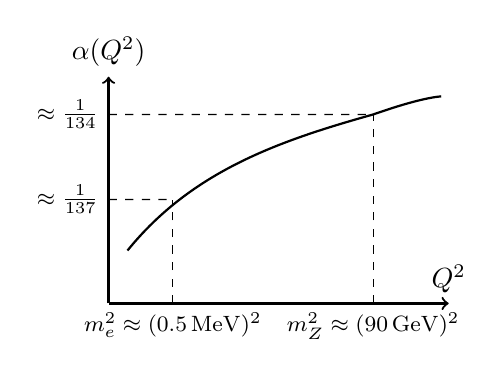
\begin{tikzpicture}[scale=0.48]
    
        % Assi
        \draw[->, thick] (0,0) -- (9,0) node[above] {$Q^2$};
        \draw[->, thick] (0,0) -- (0,6) node[above] {$\alpha(Q^2)$};
        
        % Curva
        \draw[thick]
            (0.5,1.4)
            .. controls (2.2,3.5) and (4.5,4.3)
            .. (7,5.0)
            .. controls (8,5.35) and (8.5,5.45)
            .. (8.8,5.48);
        
        % Punti scelti SULLA curva
        \coordinate (A) at (1.7,2.75);
        \coordinate (B) at (7,5.0);
        
        % Linee tratteggiate verticali
        \draw[dashed] (A |- 0,0) -- (A);
        \draw[dashed] (B |- 0,0) -- (B);
        
        % Linee tratteggiate orizzontali
        \draw[dashed] (0,2.75) -- (A);
        \draw[dashed] (0,5.0) -- (B);
        
        % Etichette asse y
        \node[left] at (0,2.75)
        {\footnotesize$\approx \frac{1}{137}$};
        
        \node[left] at (0,5.0)
        {\footnotesize$\approx \frac{1}{134}$};
        
        % Etichette asse x
        \node[below, align=center] at (1.7,0)
        {\footnotesize$m_e^2 \approx (0.5\,\mathrm{MeV})^2$};
        
        \node[below, align=center] at (7,0)
        {\footnotesize$m_Z^2 \approx (90\,\mathrm{GeV})^2$};

    \end{tikzpicture}
    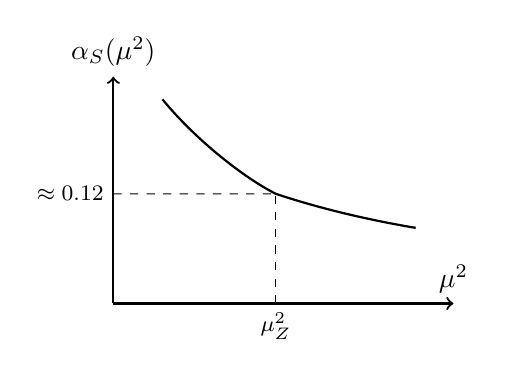
\begin{tikzpicture}[scale=0.48]
        
        % Assi
        \draw[->, thick] (0,0) -- (9,0) node[above] {$\mu^2$};
        \draw[->, thick] (0,0) -- (0,6) node[above] {$\alpha_S(\mu^2)$};
        
        % Curva decrescente (QCD running coupling)
        \draw[thick]
            (1.3,5.4)
            .. controls (2.2,4.3) and (3.5,3.3)
            .. (4.3,2.9)
            .. controls (5.5,2.5) and (6.8,2.2)
            .. (8.0,2.0);
        
        % Punto sulla curva in M_Z^2
        \coordinate (A) at (4.3,2.9);
        
        % Linea tratteggiata verticale
        \draw[dashed] (A |- 0,0) -- (A);
        
        % Linea tratteggiata orizzontale
        \draw[dashed] (0,2.9) -- (A);
        
        % Etichetta asse y
        \node[left] at (0,2.9)
        {\footnotesize$\approx 0.12$};
        
        % Etichetta asse x
        \node[below] at (4.3,0)
        {\footnotesize$\mu_Z^2$};
    \end{tikzpicture}
    \caption{trend of the coupling: (i) $\alpha(Q^2)$ in QED; (ii) $\alpha_S(\mu^2)$ in QCD.}
    \label{fig: QED and QCD coupling trend}
\end{figure}
\begin{obs}
    The running coupling has a pole at 
    \begin{equation}
        1 + \frac{b_0}{4\pi}\alpha(\mu_0)\log{\frac{\mu_L^2}{\mu_0^2}} = 0,
    \end{equation}
    where $\mu_L^2$ is the location of the Landau pole. In QED, we find that $\mu_L^{(QED)} \approx m_e\exp{(650)}$ and so way above any physical scale. For QCD, we find that the Landau pole is inside the confined region where $\alpha_S > 1$, namely $\mu_L^{(QCD)} = \mu_z\exp{[-2\pi/b_0\alpha_S(\mu_z)]} \approx \SI{250}{\MeV}$ for $n_f = 3$ active flavours.
\end{obs}
Analytic solutions to the running coupling at higher orders are not available in general, however numerical solutions may be obtained. We may find analytic expressions when keeping only the dominant logarithmic contributions
\begin{equation}
    \begin{split}
        \mu\frac{d\alpha}{d\mu} &= -\alpha\bigg[\frac{\alpha}{2\pi}b_0 + \bigg(\frac{\alpha^2}{2\pi}\bigg)^2b_1 + o(\alpha^3)\bigg] \\
        &= -\alpha^2\beta_0\bigg[1 + \alpha\frac{\beta_1}{\beta_0} + o(\alpha^2)\bigg],
    \end{split}
\end{equation}
where $\beta_k \equiv b_k/(2\pi)^{k + 1}$, thus 
\begin{equation}
    -\frac{d\mu}{\mu} = \frac{d\alpha}{\alpha^2\beta_0}\frac{1}{1 + \alpha\beta_1/\beta_0},
\end{equation}
which integrated gives
\begin{equation}
    -\log{\frac{\mu}{\mu_0}} = C - \frac{1}{\beta_0\alpha} - \frac{\beta_1}{\beta_0^2}\bigg[\log{(\alpha)} - \log{\bigg(1 + \alpha\frac{\beta_1}{\beta_0}\bigg)}\bigg],
\end{equation}
where $C$ is a constant of integration. We can find the solution iteratively. First set $\beta_1 = 0$ and choose $C$ such that 
\begin{equation}
    -\log{\frac{\mu}{\Lambda}} = -\frac{1}{\alpha\beta_0} \equiv -L,\quad C \equiv \log{\frac{\mu_0}{\Lambda}}.
\end{equation}
Now we take the leading limit of the two loop equation, correcting the integration constants 
\begin{equation}
    C = \log{\bigg(\frac{\mu_0}{\Lambda}\bigg)} - \frac{2\beta_1}{\beta_0}\log{\beta_0},
\end{equation}
which leads, substituting $\alpha = 1/\beta_0 L$ into the arguments of the logarithms and expanding, to 
\begin{equation}
    -L = -\frac{1}{\alpha\beta_0} + \frac{\beta_1}{\beta_0^2}\log{L},
\end{equation}
thus 
\begin{equation}
    \alpha = \frac{1}{\beta_0L}\bigg(1 - \frac{\beta_1}{\beta_0^2}\frac{\log{L}}{L}\bigg) + o\bigg(\frac{1}{L^2}\bigg).
\end{equation}
In QCD one finds that 
\begin{equation}
    b_1 = \frac{34}{3}C_A^2 - \frac{20}{3}C_AT_Rn_f - 4C_FT_Rn_f
\end{equation}
and the effect at 2-loops to 1-loop running can be between 1\% and 2\% for modern collider energy scales. 

We have previously seen the behaviour of the $\beta$ function for $\alpha \ll 1$, but what happens for larger values of $\alpha$? It is possible that $\beta'(\alpha) = 0$ at some point and we find $\beta(\alpha_*) = 0$ where $\alpha_* = 0$, as shown in figure \ref{fig: IR and UV fixed points}. If we assume such a point does exists we can infer the properties of the theory close to the fixed point; in fact, take $\beta(\alpha) = -B(\alpha - \alpha_*)$ close to $\alpha_*$ where $B$ is a constant, thus 
\begin{equation}
    \begin{split}
        \int_{\alpha(\mu)}^{\alpha(|p|)}\frac{d\alpha}{\alpha - \alpha_*} &= B\log{\frac{|p|}{\mu}} \\
        \log{\bigg[\frac{\alpha(|p|) - \alpha_*}{\alpha(\mu) - \alpha}\bigg]} &= \log{\bigg(\frac{|p|}{\mu}\bigg)^{-B}} \\
        \alpha(|p|) &= \alpha_* + [\alpha(\mu) - \alpha_*]\bigg(\frac{|p|}{\mu}\bigg)^{-B},
    \end{split}
\end{equation}
for some scales $|p|$ and $\mu$, so we find an exact solution to the evolution of the coupling. We can also look at the solution to the 2-point function from the Callan-Symanzik equation, namely by taking $\gamma(\alpha[|p|;\alpha(\mu)]) \equiv \gamma_*$ so that
\begin{equation}
    \begin{split}
        \tilde{G}_2(p^2,\mu^2,\alpha_*) = -\frac{i}{p^2}g_2'(\alpha_*)\exp{\bigg(2\int_\mu^{|p|}\frac{d|p'|}{|p'|}\gamma_*\bigg)} = -\frac{i}{p^2}\bigg(\frac{\mu^2}{p^2}\bigg)^{-\gamma_*}g_2'(\alpha_*).
    \end{split}
\end{equation}
\begin{figure}[h]
    \centering
    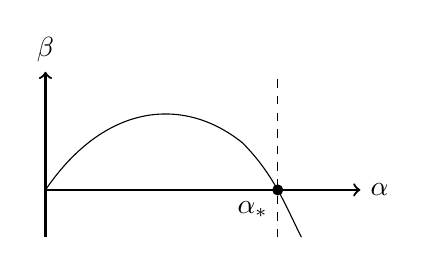
\begin{tikzpicture}[scale=0.5]
    
    % Assi
    \draw[->, thick] (0,0) -- (8,0) node[right] {$\alpha$};
    \draw[->, thick] (0,-1.2) -- (0,3.0) node[above] {$\beta$};
    
    % Curva
    \draw[]
        (0.0,0.0)
        .. controls (1.5,2.2) and (3.5,2.4)
        .. (5.0,1.2)
        .. controls (5.8,0.4) and (6.1,-0.4)
        .. (6.5,-1.2);
    
    % Linea verticale tratteggiata
    \draw[dashed] (5.9,-1.2) -- (5.9,3.0);
    
    % Label alpha*
    \node[left] at (5.9,-0.5) {$\alpha_*$};

    \fill (5.9,0.0) circle (4pt);
    
    \end{tikzpicture}
    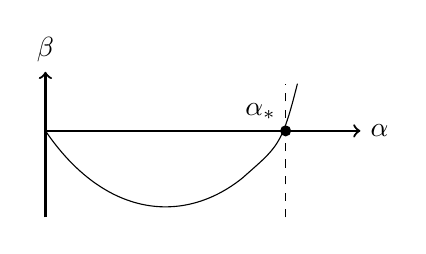
\begin{tikzpicture}[scale=0.5]
    
    % Assi
    \draw[->, thick] (0,0) -- (8,0) node[right] {$\alpha$};
    \draw[->, thick] (0,-2.2) -- (0,1.5) node[above] {$\beta$};
    
    % Curva
    \draw[]
        (0.0,0.0)
        .. controls (1.5,-2.2) and (3.5,-2.4)
        .. (5.0,-1.2)
        .. controls (5.9,-0.4) and (6.0,-0.4)
        .. (6.4,1.2);;
    
    % Linea verticale tratteggiata
    \draw[dashed] (6.1,-2.2) -- (6.1,1.2);
    
    % Label alpha*
    \node[left] at (6.1,0.5) {$\alpha_*$};

    \fill (6.1,0.0) circle (4pt);
    
    \end{tikzpicture}
    \caption{behaviour of $\beta(\alpha)$: (i) IR fixed point; (ii) UV fixed point.}
    \label{fig: IR and UV fixed points}
\end{figure}

\section{Evolution of mass parameters}
Let's consider a massive scalar theory and look at the Callan-Symanzik equation for an on-shell $S$ matrix element. In the on-shell case the factor of $n\gamma_\phi(\lambda)$ does not contribute
\begin{equation}
\label{eq: n gamma_phi contribution}
    \bigg[\mu\frac{\p}{\p \mu} + \beta(\lambda)\frac{\p}{\p \lambda} + \gamma_m(\lambda)m\frac{\p}{\p m }\bigg]S = 0,\quad S \equiv S[p_i\cdot p_j,m;\mu,\lambda(\mu)].
\end{equation}
We can normalize $S$ to form a dimensionless function $\hatS$ using the scale $\mu$, namely 
\begin{equation}
    S = \mu^{-D}\hatS\bigg[\frac{p_i\cdot p_j}{\mu^2},\frac{m^2}{\mu^2},\lambda(\mu)\bigg].
\end{equation}
We can perform a simple dimensional analysis of $S$, taking a single invariant $Q^2$ for simplicity
\begin{equation}
    \hatS \equiv \hatS\bigg[\frac{Q^2}{\mu^2},\frac{m^2}{\mu^2},\lambda(\mu)\bigg],
\end{equation}
by
\begin{equation}
\label{eq: dimensionless S function}
    \begin{split}
        0 &= \bigg(\mu\frac{\p}{\p \mu} + Q\frac{\p}{\p Q} + m\frac{\p}{\p m} + D\bigg)S \\
        &= 2\bigg(\mu^2\frac{\p}{\p \mu^2} + Q^2\frac{\p}{\p Q^2} + m^2\frac{\p}{\p m^2} + \frac{D}{2}\bigg)(\mu^2)^{-D/2}\hatS \\
        &= 2(\mu^2)^{-D/2}\bigg(\mu^2\frac{\p}{\p \mu^2} + Q^2\frac{\p}{\p Q^2} + m^2\frac{\p}{\p m^2} \bigg)(\mu^2)^{-D/2}\hatS.
    \end{split}
\end{equation}
The difference between equation \eqref{eq: dimensionless S function} and equation \eqref{eq: n gamma_phi contribution} gives
\begin{equation}
    \bigg\{Q\frac{\p}{\p Q} - \beta(\lambda)\frac{\p}{\p\lambda} + [1 - \gamma_m(\lambda)]m\frac{\p}{\p m} + D\bigg\}S = 0.
\end{equation}
This latter equation may be solved using the same method used for the Callan-Symanzik equation in which both coupling and mass run with energy, namely where $\hat{\lambda}(Q;\lambda)$ satisfy 
\begin{equation}
    Q\frac{d\hat{\lambda}}{dQ} = \beta(\hat{\lambda})
\end{equation}
and $\hat{m}(Q;\lambda)$ satisfy 
\begin{equation}
    Q\frac{d\hat{m}}{dQ} = -[1 - \gamma_m(\hat{\lambda})]\hat{m},
\end{equation}
where $\hat{\lambda}$ runs from the point $\lambda$ where we have measured the coupling and fixed the renormalization scheme. The mass run from the value of the mass at the same renormalization scale $\mu$, for example $\hat{\lambda}(\mu;\lambda) = \lambda(\mu)$ and $\hat{m}(\mu;\lambda) = m(\mu)$, then
\begin{equation}
    \hat{m}(Q;\lambda) = m(\mu)\exp{\bigg\{-\int_\mu^Q\frac{dQ'}{Q'}[1 - \gamma_m(\hat{\lambda})]\bigg\}}.
\end{equation}